\documentclass[11pt]{article}
%基于北京航空航天大学仪器科学与光电工程学院实验报告及课程报告排版得来,类似于毕业论文排版格式
%后续将更新毕业论文排版格式
\usepackage{graphicx,float}%使用图的宏包,使用图的浮动体宏包,引入参数H使图像紧跟当前文字
\usepackage{caption} %使用图表标题的宏包
\usepackage[colorlinks=true,pdfstartview=FitH,%
linkcolor=black,anchorcolor=violet,citecolor=magenta]{hyperref}%加载hyperref宏包,使用超链接
\usepackage{setspace}%用于设置行间距列间距等命令的宏包
\usepackage{array}%设置列表高度宽度的宏包
\usepackage{zhnumber}%使用中文数字编号的宏包
\usepackage{titlesec,titletoc}%使用标题自定义形式的宏包和使用目录自定义形式的宏包
\usepackage{siunitx}%物理学单位宏包
\usepackage{tabularx}%让表格宽度等于页面宽度
\usepackage{makecell}%单个表格单元调整的宏包
\usepackage{subfigure} %%使用子图的宏包
\usepackage[backend=biber,bibstyle=gb7714-2015,%nature,%%加载biblatex宏包,使用参考文献
citestyle=gb7714-2015%,backref=true%%其中后端backend使用biber
,url=false
]{biblatex}%标注(引用)样式citestyle,著录样式bibstyle都采用gb7714-2015样式
% \usepackage{pgfplots}%类似tikz的一个画图库,主要画统计图
\usepackage{../customStyle}
% \usepackage{customFont}%自行编写的字体命令库,基于CJK宏包
% \usepackage{bh_style}%自行编写的风格文件,基于使用习惯和格式要求
% \usepackage{math_formulate}%自行编写的数学公式命令库,基于amsmath宏包
% \usepackage{picture}%集成图形绘制库,主要包括了tikz和pgfplots两大主流宏包
% \usepackage[lite,subscriptcorrection,slantedGreek,nofontinfo]{mtpro2}%使用mathtimepro2商业字体作为数学环境,并不推荐

%biblatex宏包的参考文献数据源加载方式,注意book.bib应当与.tex文件在同一目录下,不然有可能会报错
\addbibresource[location=local]{book.bib}
% % \bibliographystyle{gbt7714-numerical}
%%% 下面的命令重定义页面边距,使其符合中文刊物习惯 %%%%
% \addtolength{\topmargin}{2.5cm}
\setlength{\oddsidemargin}{0.63cm}  % 3.17cm - 1 inch
\setlength{\evensidemargin}{\oddsidemargin}
% \setlength{\textwidth}{14.66cm}
% \setlength{\textheight}{24.00cm}    % 24.62

\graphicspath{{./fig}}

\begin{document}
{
\pagestyle{empty}
\begin{figure}
  
\includegraphics{title.jpg}
\end{figure}
\begin{center}

  \begin{figure}[h]

    \centering
    
\includegraphics[]{title.png}\par
    \vspace{4em}
    \large{\yihao\lishu{2023-2024学年第二学期}}
    \vspace{6em}
  \end{figure}

  \large{\erhao\lishu{机电仿真实验}}\par
  \large{\erhao\lishu{课程作业}}
  \vspace{8em}

  \begin{spacing}{2.0}
    \begin{tabular}{cc}


      {\xiaoerhao\lishu{班\quad \quad 级}} & {\heiti{\dlmu{SY23173}}}    \\
      {\xiaoerhao\lishu{学\quad \quad 号}} & {\heiti{\dlmu{SY2317301} }} \\
      {\xiaoerhao\lishu{姓\quad \quad 名}} & {\heiti{\dlmu{陈博非} }}       \\
      {\xiaoerhao\lishu{日\quad \quad 期}} & {\heiti{\dlmu{\today} } }   \\
    \end{tabular}
  \end{spacing}
\end{center}
\thispagestyle{empty}
}


\newpage
%手动分页
\pagenumbering{roman}

\setcounter{tocdepth}{3}
%设定目录深度                      
\tableofcontents
%列出目录
\newpage

\pagenumbering{arabic}
\setcounter{page}{1}
\section{烤箱模型}
本应用是控制一个通风烤箱的温度,热量由热电阻产生,控制电压为$V_c$温度由放在测量孔中的热电偶测量,仪表放大器产生电压$V_m $显示温度$ \theta_m$ 。在烤箱温度范围内,假定传感器和仪表放大器装置是线性的 。
\begin{figure}[H]
  \centering
  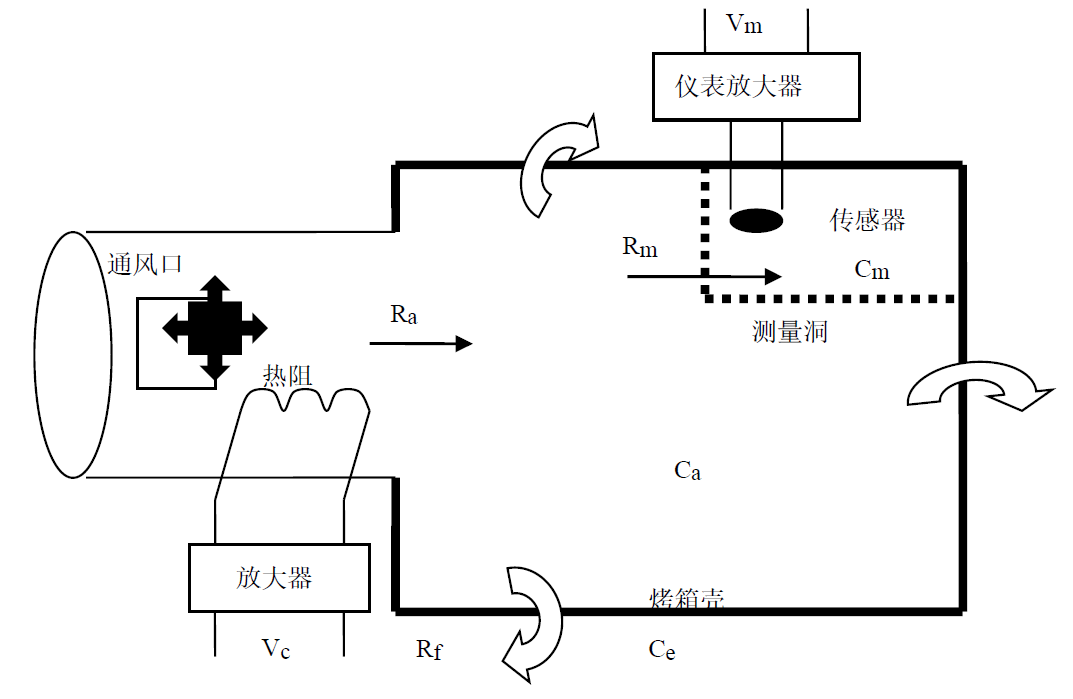
\includegraphics[width=0.8\textwidth]{烤箱结构图.png}
  \caption{烤箱结构图}
  \label{fig:烤箱结构图}
\end{figure}
此过程中包含的参数如下:
\begin{table}[H]
  \centering
  \renewcommand{\arraystretch}{1.5}
  \begin{tabular}{c|l}
    \hline
    参数符号                         & 物理意义                \\
    \hline
    $Q=k_1V_c$                   & 产生的功率               \\
    $R_a$                        & 减少导管热向机壳传播的热电阻      \\
    $C_a$                        & 机壳的热容               \\
    $R_m$                        & 头像测量洞中的烤箱热循环的热电阻    \\
    $C_m$                        & 测量洞的热容              \\
    $R_f$                        & 降低朝烤箱外热循环的泄漏电阻      \\
    $C_e$                        & 烤箱外的热容,认为非常大        \\
    $\theta_a,\theta_m,\theta_e$ & 分别代表烤箱机壳、测量洞和烤箱外的温度 \\
    $V_m=\theta_mk_2$            & 仪表放大器产生的电压          \\
    \hline
  \end{tabular}
\end{table}
\begin{figure}[H]
  \centering
  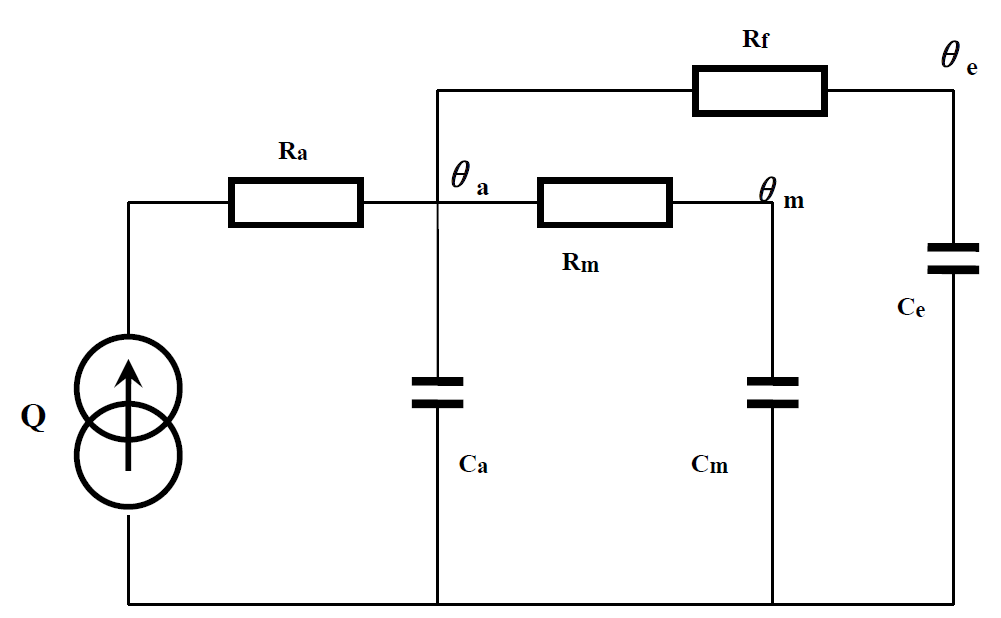
\includegraphics[width=0.8\textwidth]{等价电路图.png}
  \caption{等价电路图}
  \label{fig:等价电路图}
\end{figure}
该系统模型等价的电路图如图\ref{fig:等价电路图}所示,热力学系统可用如下方程描述:
\begin{equation}
  Q=C_a\diff{\theta_a}{t}+C_m\diff{\theta_m}{t}+\frac{\theta_a-\theta_e}{R_f}
  \label{eq:烤箱热力学方程}
\end{equation}\par
其中:
\begin{equation*}
  \theta_m=\theta_a-R_mC_m\diff{\theta_m}{t}
\end{equation*}
设定烤箱参数取如下的值:
\begin{table}[H]
  \centering
  \renewcommand{\arraystretch}{1.5}
  \caption{烤箱参数表}
  \begin{tabular}{c}
    $R_a=0.01\unit{\celsius/W}$   \\
    $R_m=3\unit{\celsius/W}$      \\
    $R_f=0.1\unit{\celsius/W}$    \\
    $Q_\mathrm{max}=5000\unit{W}$ \\
    $k_1=100\unit{W/V}$           \\
    $k_2=0.1\unit{V/\celsius}$    \\
    $C_a=5000\unit{J/\celsius}$   \\
    $C_m=10\unit{J/\celsius}$     \\
    $C_e=\infty\unit{J/\celsius}$ \\
    $\theta_e=20\unit{\celsius}$  \\
  \end{tabular}
\end{table}
\section{实验要求}
利用MWorks.Sysplorer软件对该烤箱控制系统进行仿真,设定在$Q=1000\unit{W}$、烤箱外的温度$\theta_e=20\unit{\celsius}$的情况下,要求输出控制电压$V_c$和测量电压$V_m$随时间的变化曲线,输出烤箱机温度$\theta_e$和测量洞温度$\theta_m$随时间的变化曲线。
\section{模型建立}
考虑到使用MWorks.Sysplorer软件构建控制模型应当在频域或者状态变量空间下进行,因此首先对热力学微分方程\ref{eq:烤箱热力学方程}进行拉普拉斯变换:
\begin{align*}
  Q(s)        & =sC_a\Theta_a(s)+sC_m\Theta_m(s)+\frac{\Theta_a(s)-\Theta_e(s)}{R_f} \\
  \Theta_m(s) & =\Theta_a(s)-sR_mC_m\Theta_m(s)                                      \\
  Q(s)        & =k_1V_c(s)                                                           \\
  V_m(s)      & =\Theta_m(s)k_2
  \label{eq:烤箱热力学方程拉普拉斯}
\end{align*}\par
联立以上式子,得到烤箱控制系统的各个量的复频域响应函数:
\begin{align*}
  \Theta_m(s) & =\frac{\Theta_e(s)+Q(s)R_f}{1+(C_aR_f+C_mR_f+R_mC_m)s+C_aR_mC_mR_fs^2}              \\
  \Theta_a(s) & =\frac{[\Theta_e(s)+Q(s)R_f](1+sR_mC_m)}{1+(C_aR_f+C_mR_f+R_mC_m)s+C_aR_mC_mR_fs^2} \\
  V_m(s)      & =\frac{\Theta_e(s)+Q(s)R_f}{1+(C_aR_f+C_mR_f+R_mC_m)s+C_aR_mC_mR_fs^2}k_2           \\
  V_c(s)      & =\frac{Q(s)}{k_1}
\end{align*}\par
以$Q(t)=1000U(t)/\unit{W}$和$\Theta_e(t)=20/\unit{\celsius}$作为输入的激励信号,代入各个参数的值,作一次小量近似,可得到系统的频域响应函数为:
\begin{align*}
  \Theta_m(s) & =\frac{\Theta_e(s)+Q(s)R_f}{1+531s+15000s^2}\approx\frac{\Theta_e(s)+\frac{1}{10}Q(s)}{(1+500s)(1+30s)} \\
  \Theta_a(s) & =\frac{(1+30s)[\Theta_e(s)+Q(s)R_f]}{1+531s+15000s^2}\approx\frac{\Theta_e(s)+\frac{1}{10}Q(s)}{1+500s}     \\
  V_m(s)      & =\frac{\Theta_e(s)+Q(s)R_f}{1+531s+15000s^2}\frac{1}{10}   \approx\frac{\Theta_e(s)+\frac{1}{10}Q(s)}{(1+500s)(1+30s)}\frac{1}{10} \\
  V_c(s)      & =\frac{Q(s)}{100}
\end{align*}\par
由此可知系统的框图如图\ref{fig:系统框图}所示:
\begin{figure}[H]
  \begin{center}
    \begin{tikzpicture}[
      terminal/.style={
          % The shape:
          rectangle,minimum size=6mm,rounded corners=3mm,
          % The rest
          very thick,draw=black!50,
          top color=white,bottom color=black!20,
          font=\songti},>={Stealth[round]},thick,black!50,text=black,
      every new ->/.style={shorten >=1pt},
      graphs/every graph/.style={edges=rounded corners},point/.style={inner sep=0pt,minimum size=0pt},
      hv path/.style={to path={-| (\tikztotarget)}},
      vh path/.style={to path={|- (\tikztotarget)}}]

      \matrix[row sep=5mm,column sep=5mm] {
        & \node(Q_input) [point]     {$Q(s)$     }    ;                                   & \node(k1) [terminal] {$\displaystyle \frac{1}{100} $}; & \node(Vc_s)[point]{$\quad\quad$}; &  & &  &  &   & \\
        % First row:
                                                  &\node(Rf) [terminal] {$\displaystyle \frac{1}{10} $};                                    &  &  &  & \node(theta_a){$\Theta_a(s)$}; &  &  &   & \\
        % Second row:
        \node(theta_input)[point]{$\Theta_e(s)$}; & \node(error)[terminal]{};                                                          & \node(second_imped) [terminal] {$\displaystyle\frac{1}{500s+1}$};   & \node(theta_a_south)[point]{};
                                                  &
                                                  & \node(first_imped) [terminal] {$ \displaystyle\frac{1}{30s+1} $}; &
                                                  & \node(feedback)[point]{};                                                          & \node(k2) [terminal] {$\displaystyle \frac{1}{10}$};  & \node(Vm_s)[point]{$V_m(s)$};                                                     \\
        % Third row:
                                                  &                                                                                    &                                                                           &                                   &  &                                &  &  &     \\
      };
      \coordinate[label=$\Theta_m(s)$,xshift=16mm,yshift=-1mm](thetam) at (first_imped);
      \coordinate[label=$V_c(s)$,xshift=16mm,yshift=-1mm](vcs) at (k1);
      \node(northeast_error) at
      ($ (error) ! {5mm} ! 45:(first_imped) $) {};
      \draw [color=black!50,very thick] (northeast_error)--($ (northeast_error) ! 8mm ! (error) $);
      \node(southeast_error) at
      ($ (error) ! {5mm} ! -45:(first_imped) $) {};
      \draw [color=black!50,very thick] (southeast_error)--($ (southeast_error) ! 8mm ! (error) $);
      \graph{
      (theta_input)->(error)->(second_imped)->(first_imped)->(k2)->(Vm_s);
      (Q_input)->(Rf)->(error);
      (theta_a_south)->[vh path](theta_a);
      (Q_input)->(k1)->(Vc_s);
      ()
      };
    \end{tikzpicture}
    \caption{系统框图}
    \label{fig:系统框图}
  \end{center}
\end{figure}
由此可以使用MWorks.Sysplorer软件构建系统的框图如下:
\begin{figure}[H]
  \centering
  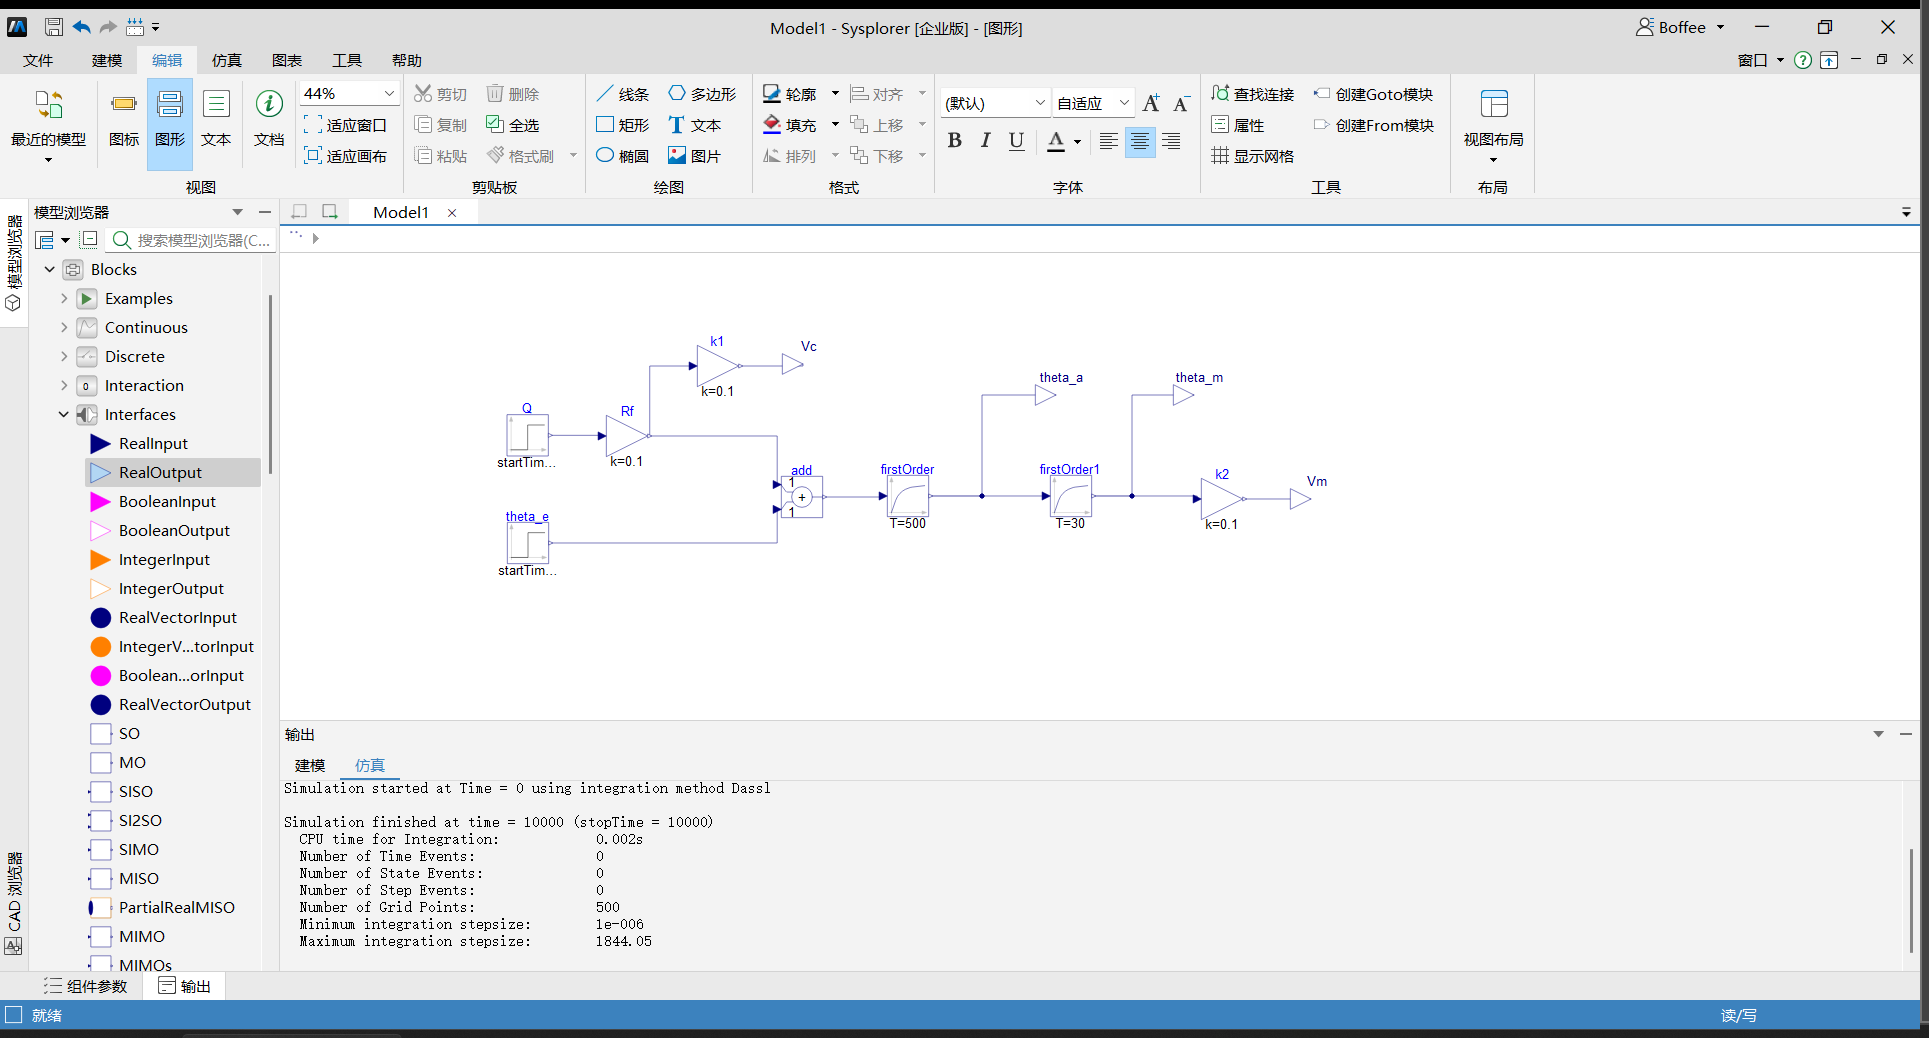
\includegraphics[width=1.0\textwidth]{仿真软件框图.png}
  \caption{仿真软件框图}
  \label{fig:仿真软件框图}
\end{figure}
\section{仿真结果}
\subsection{阶跃温度输入}
选取外界温度和功率均为阶跃输入函数,则有:
\begin{align*}
 \theta_e(t)=20U(t),\quad Q(t)=1000U(t)
\end{align*}\par
仿真结果为:
\begin{figure}[H]
  \centering
  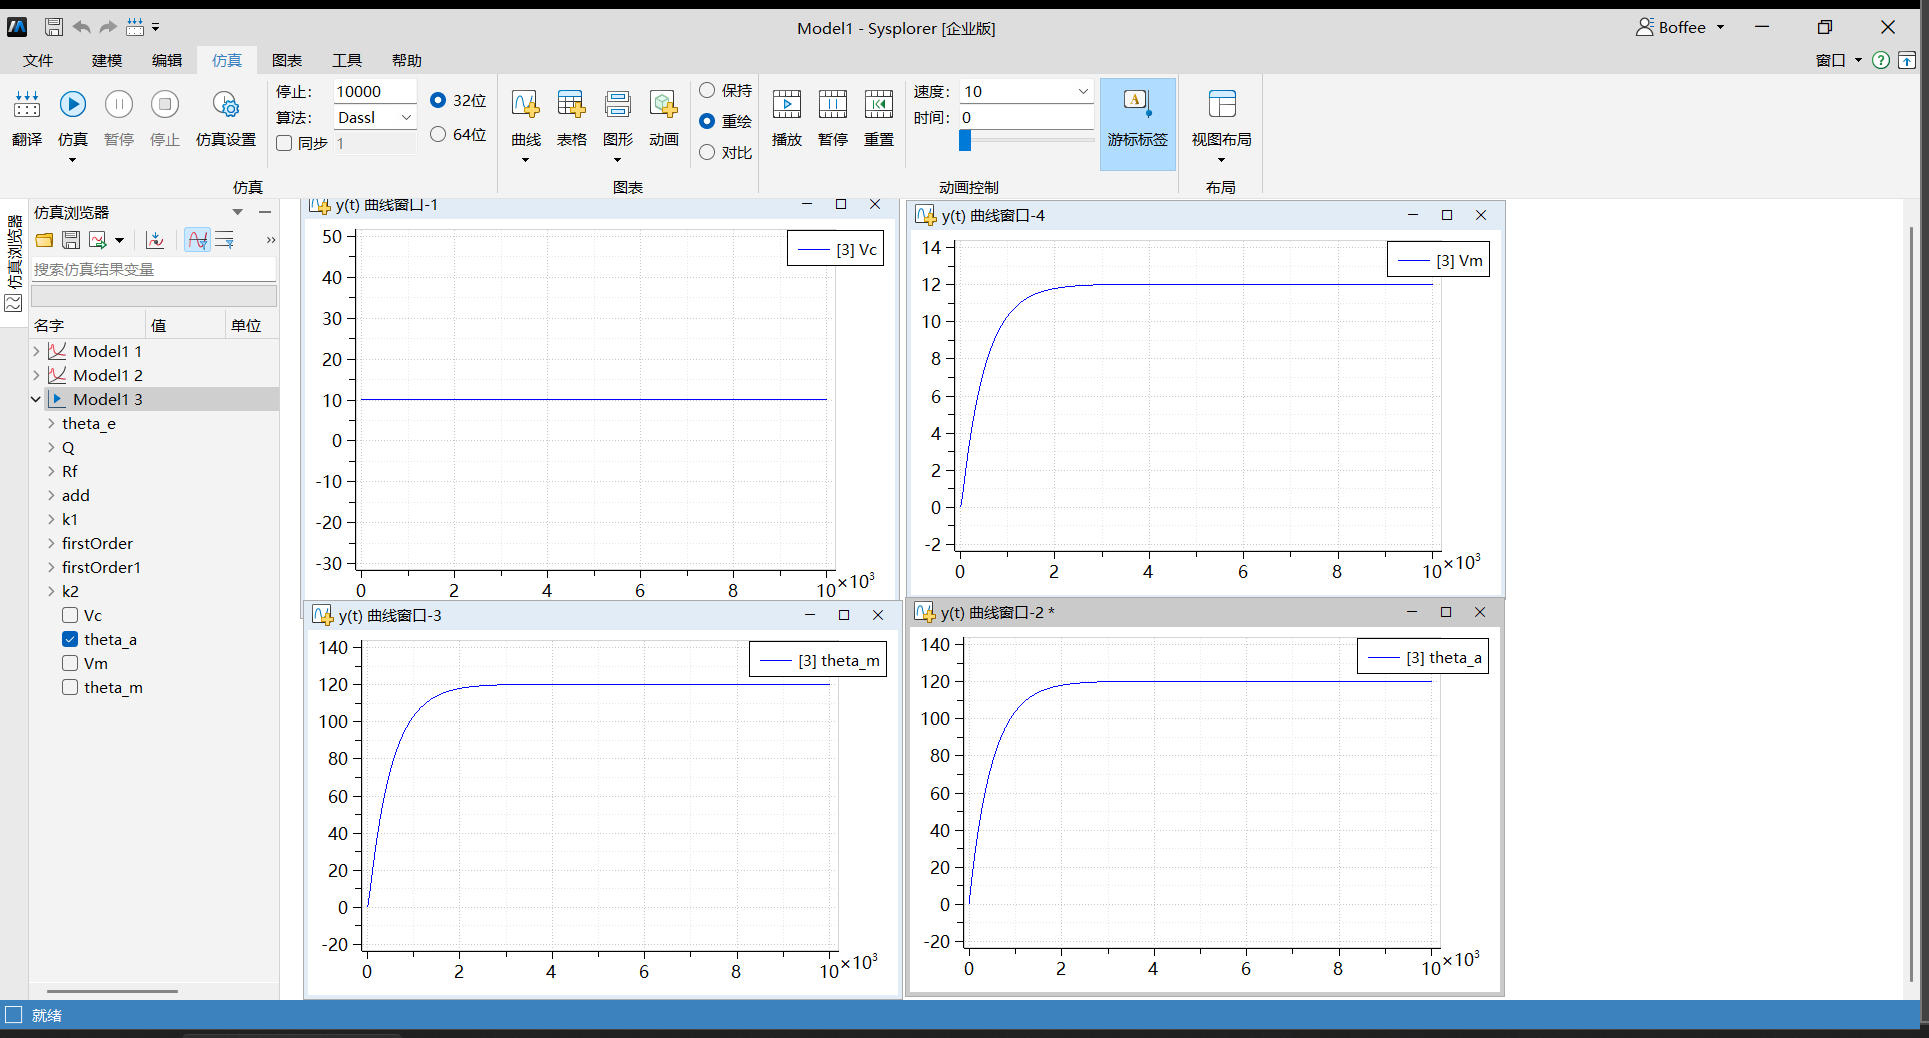
\includegraphics[width=1.0\textwidth]{阶跃输入仿真.png}
  \caption{阶跃输入仿真结果}
  \label{fig:阶跃输入仿真}
\end{figure}
\subsection{正弦温度输入}
选取功率为正弦输入函数,其波动范围为$500\unit{W}$,波动频率为$0.001\unit{Hz}$,而外界温度$\theta_e(t)$仍保持为阶跃函数,则有:
\begin{align*}
  \theta_e(t)=20U(t),\quad Q(t)=1000+500\sin(\frac{2\pi}{1000}t)U(t)
\end{align*}\par
仿真软件构建的框图如图\ref{fig:正弦仿真框图}所示:
\begin{figure}[H]
  \centering
  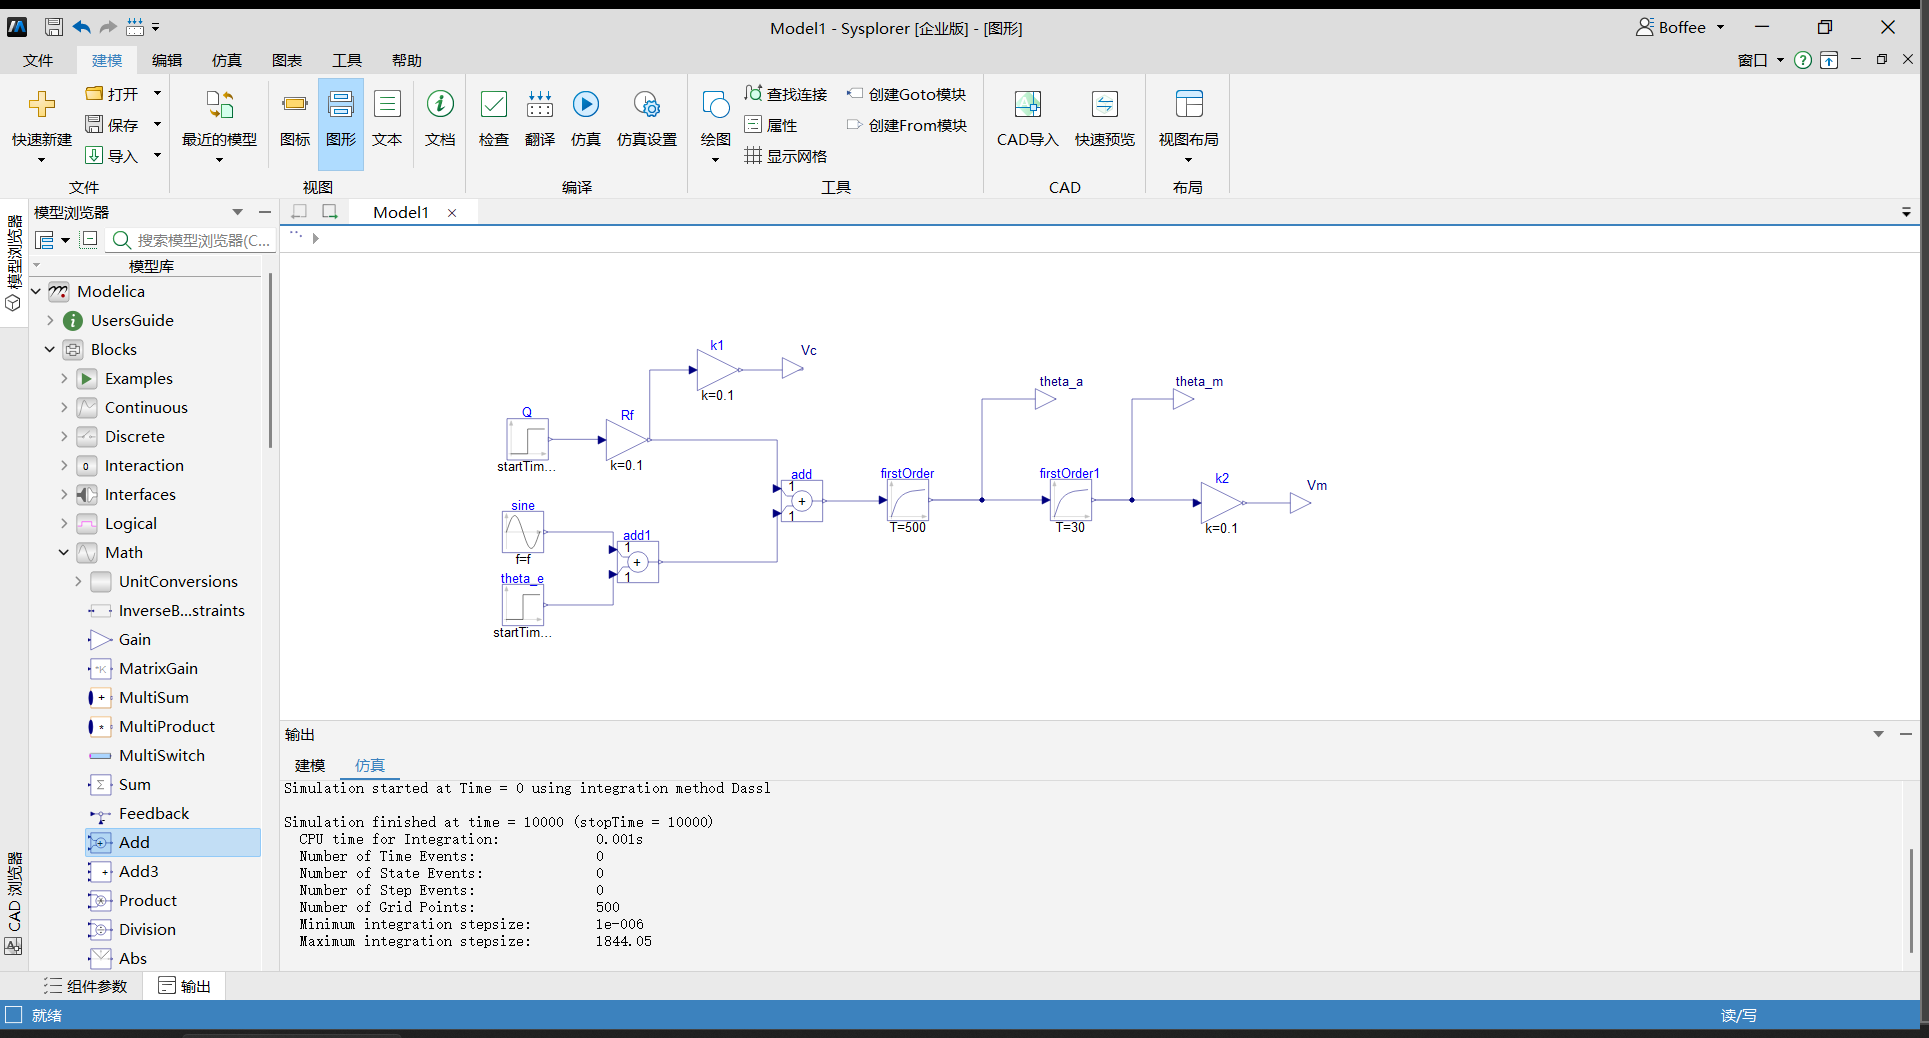
\includegraphics[width=1.0\textwidth]{正弦仿真框图.png}
  \caption{正弦仿真框图}
  \label{fig:正弦仿真框图}
\end{figure}
仿真结果为:
\begin{figure}[H]
  \centering
  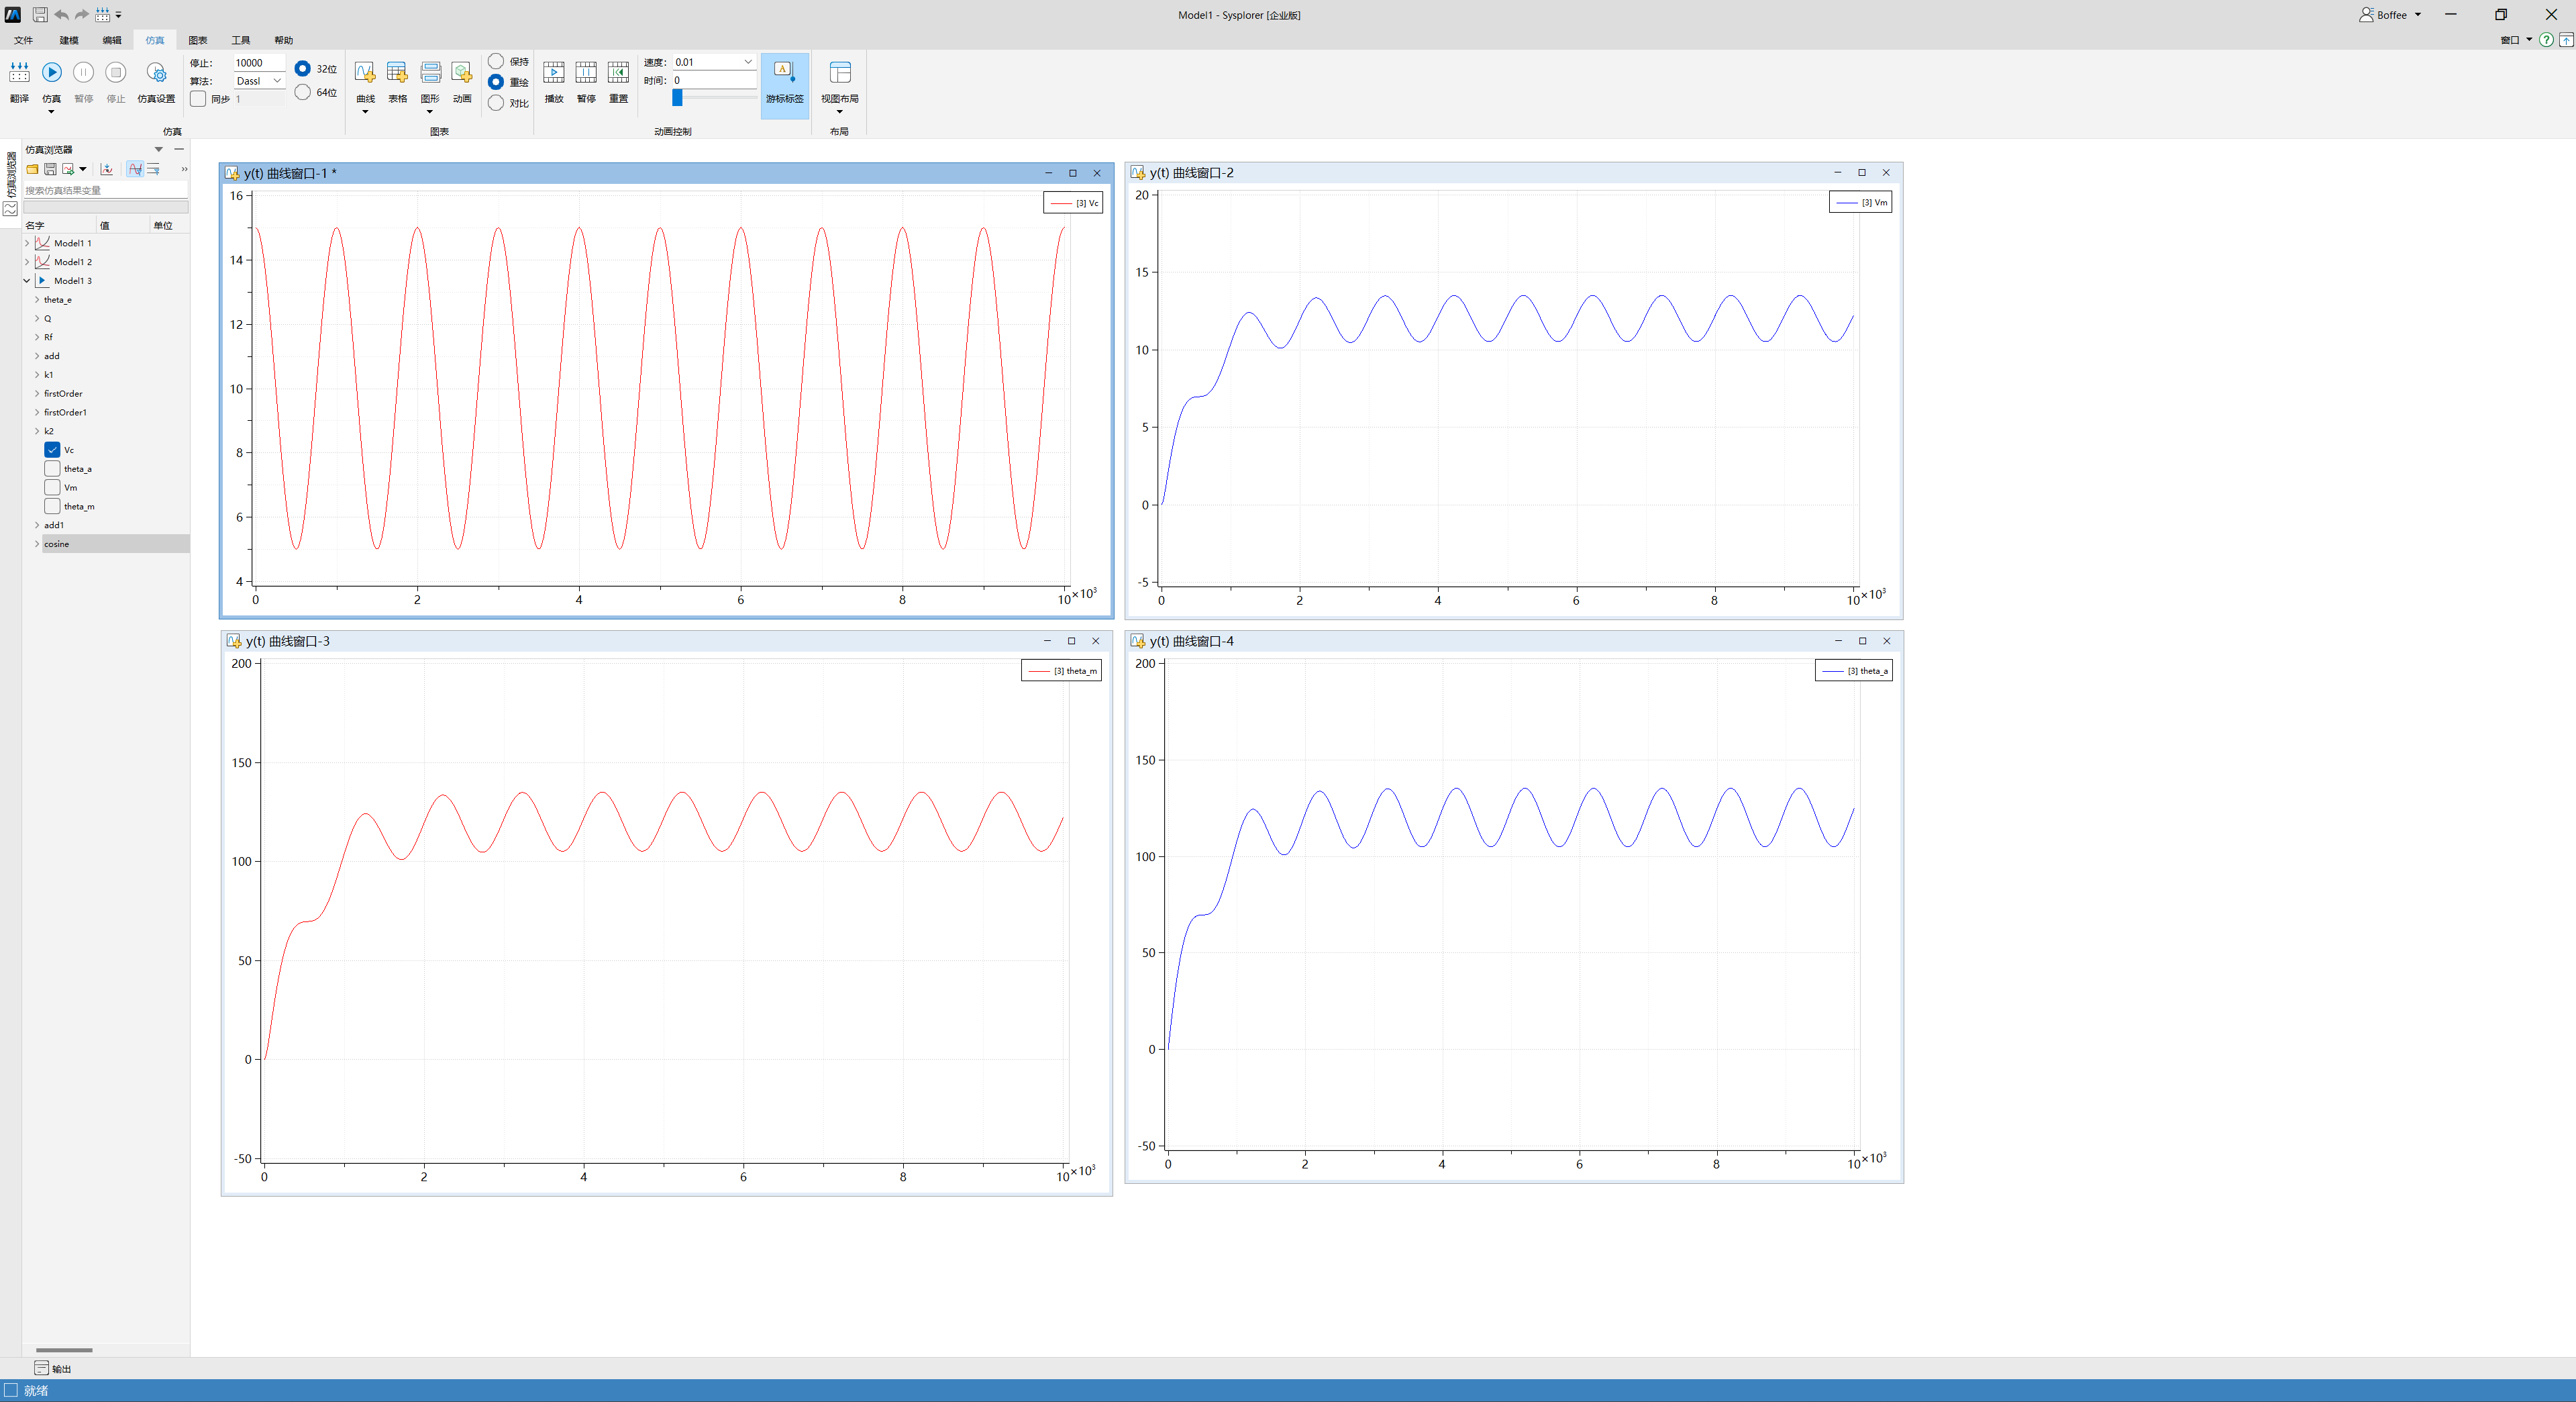
\includegraphics[width=1.0\textwidth]{正弦温度输入仿真50,0.001.png}
  \caption{正弦温度输入仿真结果$500\unit{W},1\unit{mHz}$}
  \label{fig:正弦温度输入仿真50,0.001}
\end{figure}
修改输入的正弦温度波动范围为$100\unit{W}$,仿真结果如图\ref{fig:正弦温度输入仿真100,0.001}所示:
\begin{figure}[H]
  \centering
  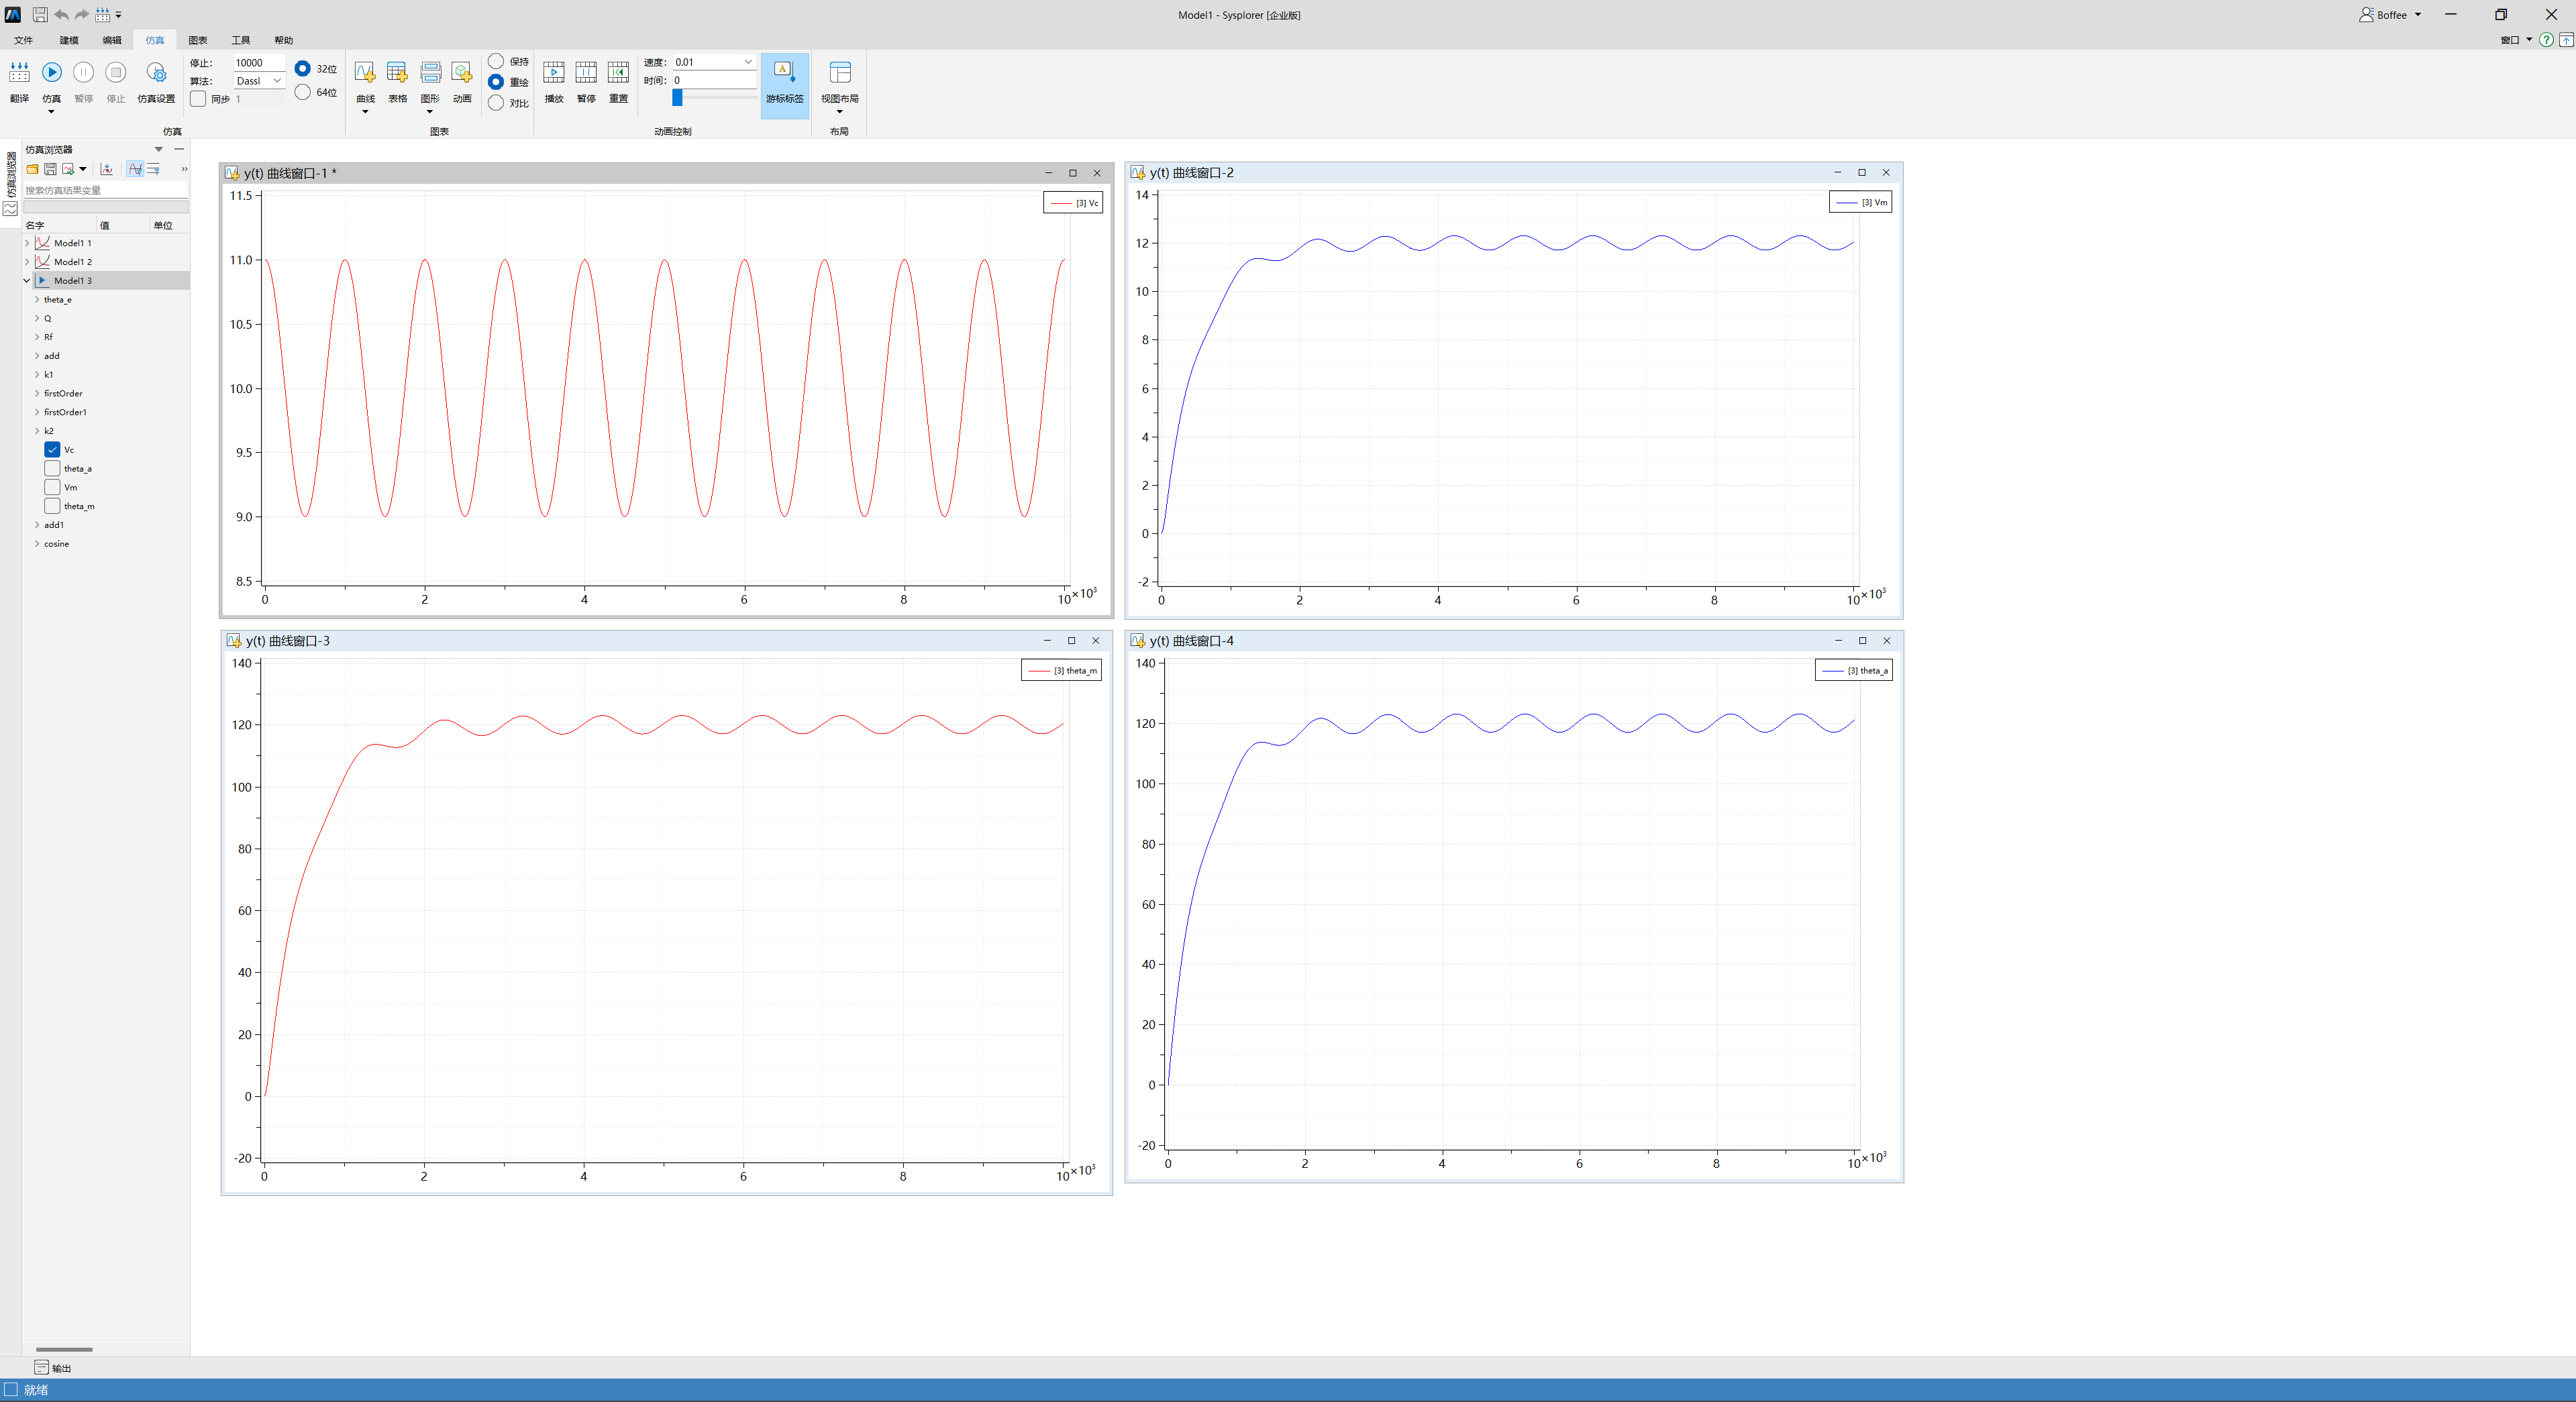
\includegraphics[width=1.0\textwidth]{正弦温度输入仿真100,0.001.png}
  \caption{正弦温度输入仿真结果$100\unit{W},1\unit{mHz}$}
  \label{fig:正弦温度输入仿真100,0.001}
\end{figure}
修改正弦输入的频率为$10\unit{Hz}$,仿真结果如图\ref{fig:正弦温度输入仿真100,10}所示:
\begin{figure}[H]
  \centering
  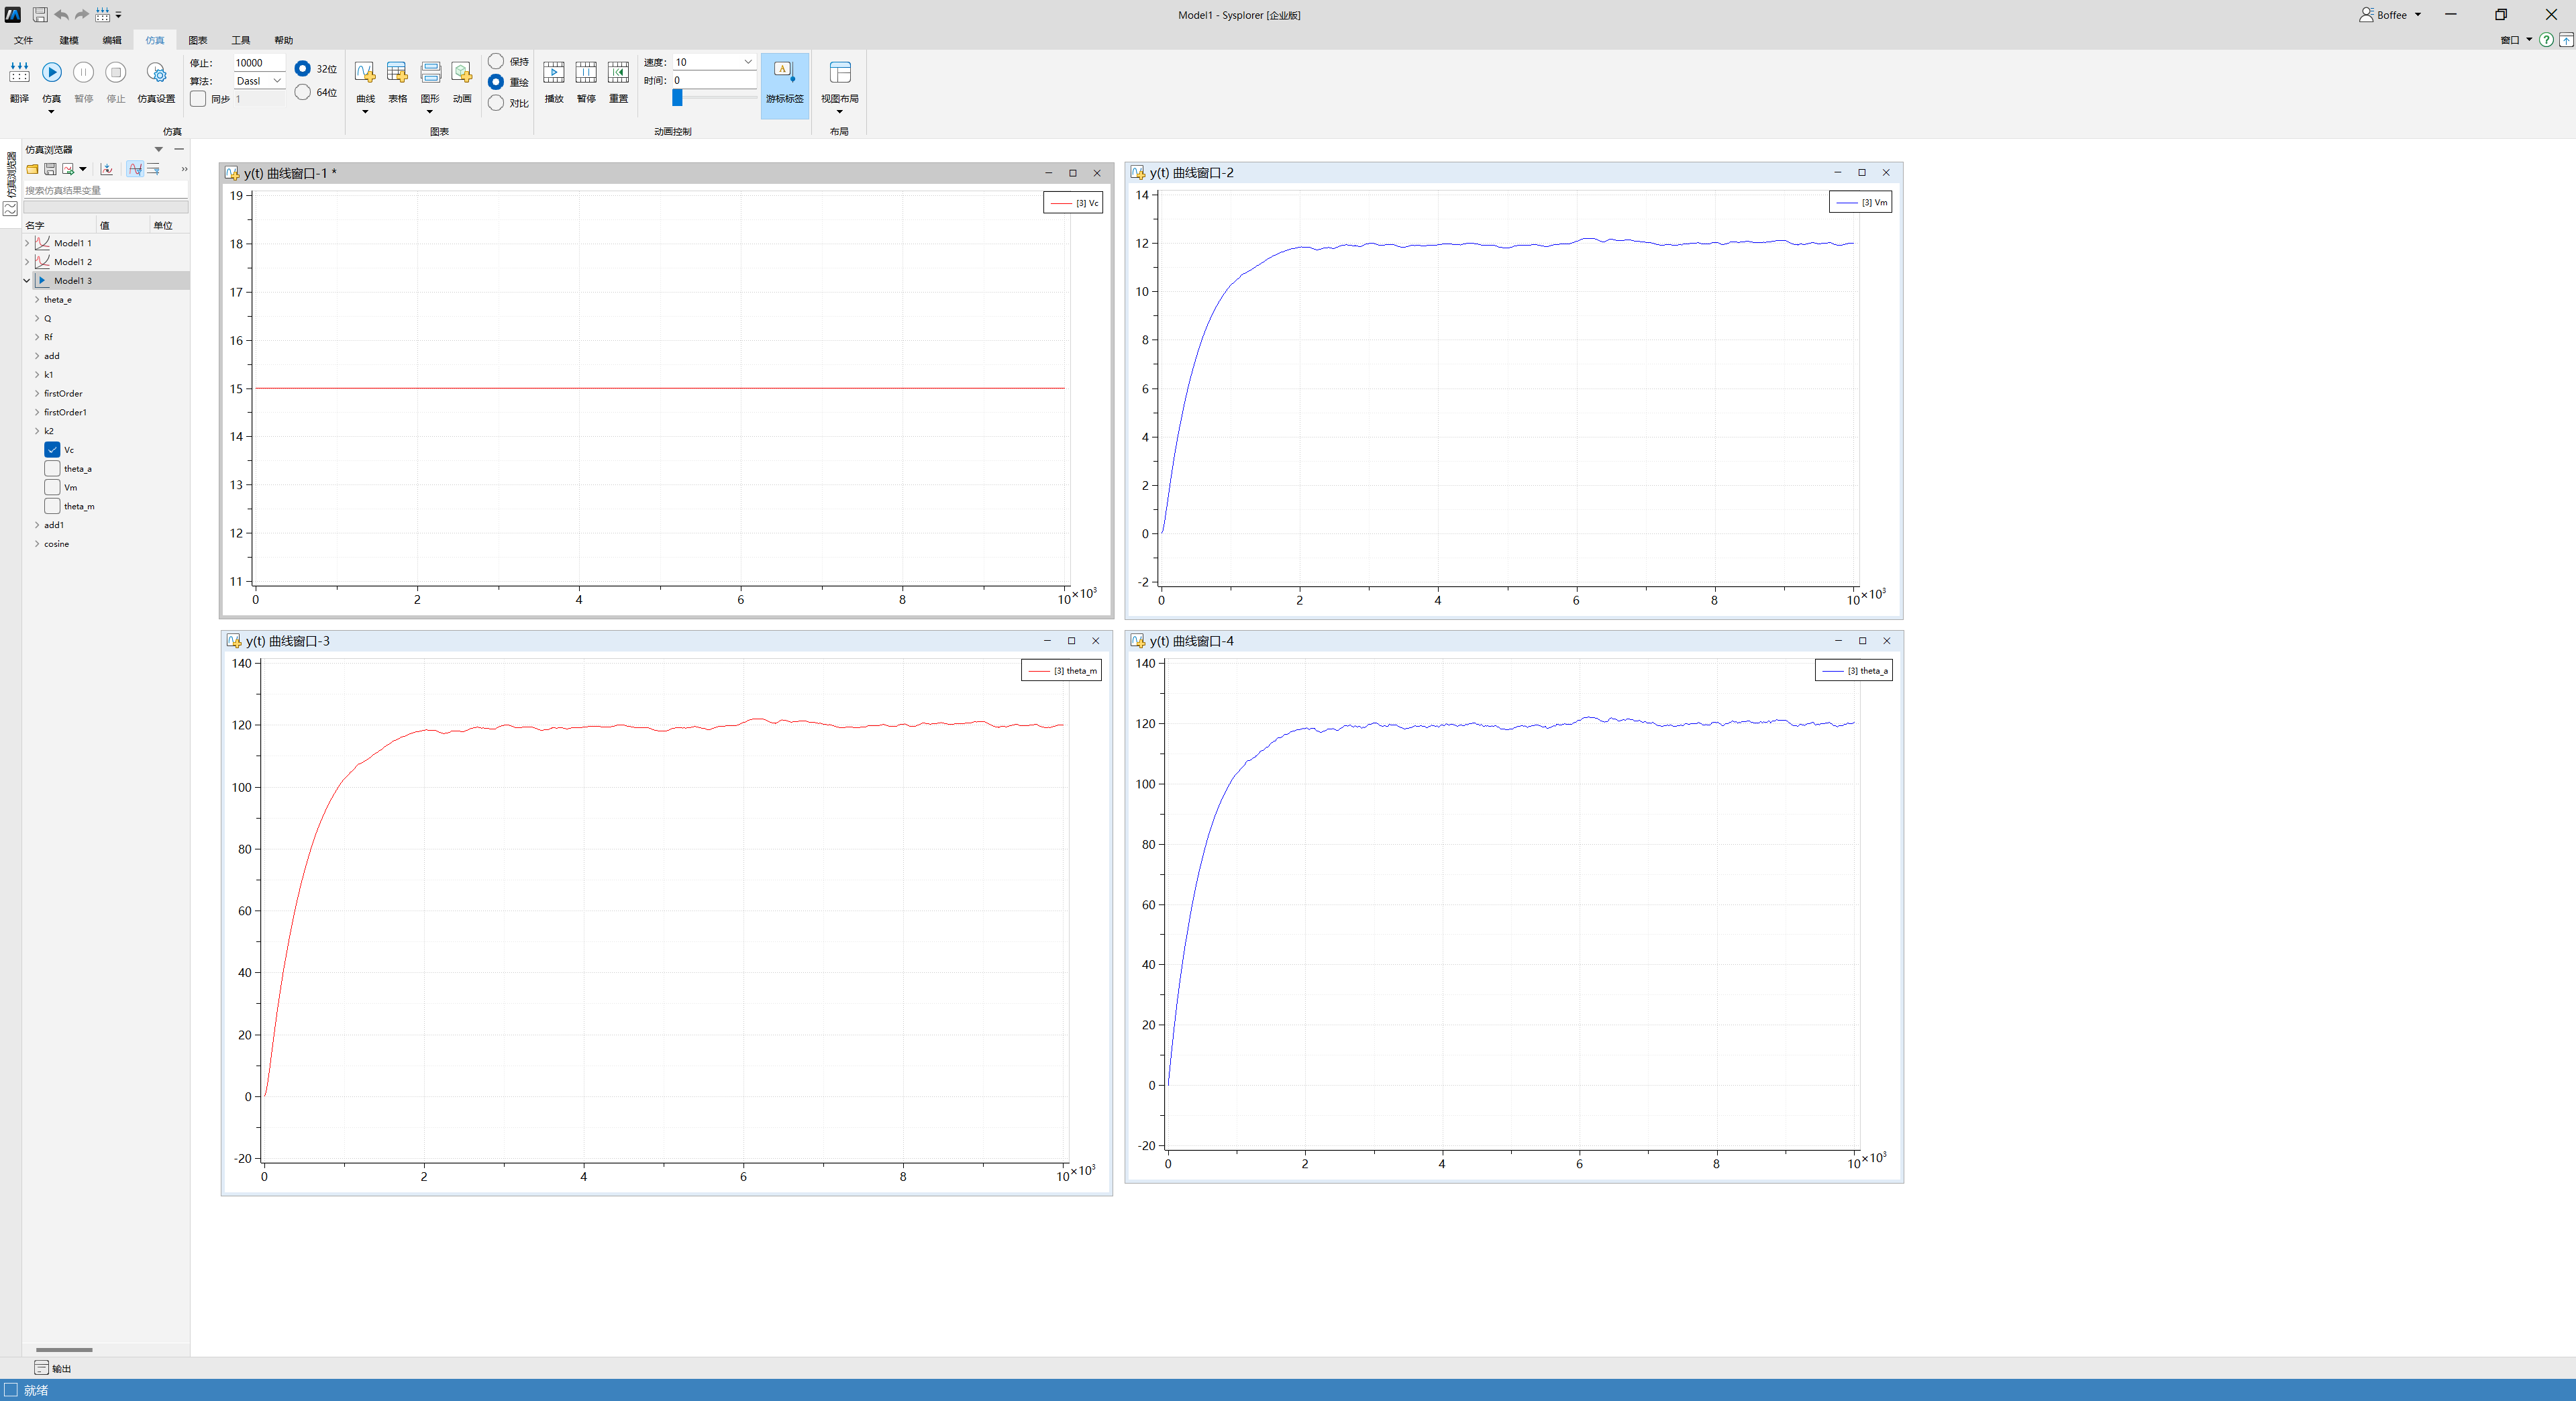
\includegraphics[width=1.0\textwidth]{正弦温度输入仿真100,10.png}
  \caption{正弦温度输入仿真结果$500\unit{W},10\unit{Hz}$}
  \label{fig:正弦温度输入仿真100,10}
\end{figure}
\section{结论}
经过上述仿真,可以发现国产软件Mworks在电气仿真方面的功能比较强大,用户界面也友好易于使用,极大地兼容了Matlab的Simulink的使用习惯。但是也存在一定的问题,例如在图\ref{fig:正弦温度输入仿真100,10}中可以看到,当仿真输入的正弦波动曲线频率较高时,在大步长时间范围内的显示结果不全;且图窗用户界面难以调整放缩分辨率,不能查看响应曲线的细节。

因此仿真软件国产化仍然有着较多的工作需要完成。
\newpage
\printbibliography[heading=bibliography,title=参考文献]
\end{document}
